% !TEX program = xelatex
\documentclass[11pt,a4paper]{article}
% !TEX program = xelatex
\usepackage[a4paper,top=23mm,bottom=24mm,left=21mm,right=21mm,headheight=15pt]{geometry}
\usepackage{fontspec}
\usepackage{kotex}
\usepackage{graphicx}
\usepackage{booktabs}
\usepackage{array}
\usepackage{tabularx}
\usepackage{makecell}
\usepackage[inline]{enumitem}
\usepackage{setspace}
\usepackage{xcolor}
\usepackage{fancyhdr}
\usepackage{lastpage}
\usepackage{calc}
\usepackage{needspace}
\usepackage{hyperref}

\defaultfontfeatures{Ligatures=TeX}

% Korean exam style: body and headings are set in a true Myeongjo/Batang-style face.
% This avoids sans-serif fallback that can look like Gulim in PDF viewers.
\setmainfont{Linux Libertine O}
\setsansfont{Noto Sans}
\setmonofont{DejaVu Sans Mono}
\setmainhangulfont{NanumMyeongjo}
\setsanshangulfont{NanumBarunGothic}

% Linguistic forms and IPA.
\newfontfamily\lingfont{Charis SIL}[Scale=MatchLowercase]
\hypersetup{colorlinks=true, linkcolor=black, urlcolor=black, pdfborder={0 0 0}}
\definecolor{RuleGray}{HTML}{4F4F4F}
\definecolor{LightRuleGray}{HTML}{B7B7B7}

\setlength{\parindent}{0pt}
\setlength{\parskip}{0.36em}
\setlength{\tabcolsep}{0.62em}
\renewcommand{\arraystretch}{1.16}
\raggedbottom
\sloppy
\emergencystretch=2em

\pagestyle{fancy}
\fancyhf{}
\fancyhead[L]{\footnotesize\bfseries 2025-2학기 특별 세션 1}
\fancyhead[R]{\footnotesize\bfseries 미니 언어학 올림피아드}
\fancyfoot[C]{\footnotesize \thepage\,/\,\pageref*{LastPage}}
\renewcommand{\headrulewidth}{0.35pt}
\renewcommand{\footrulewidth}{0pt}

\fancypagestyle{plain}{%
  \fancyhf{}%
  \fancyfoot[C]{\footnotesize \thepage\,/\,\pageref*{LastPage}}%
  \renewcommand{\headrulewidth}{0pt}%
  \renewcommand{\footrulewidth}{0pt}%
}

\newcommand{\term}[1]{{\lingfont\bfseries #1}}
\newcommand{\ipa}[1]{{\lingfont [#1]}}
\newcommand{\blankko}[1]{(\textbf{#1})}
\newcommand{\subq}[1]{\par\smallskip\noindent\textbf{(#1)}\quad}
\newcommand{\credit}[1]{\nobreak\hspace{1em}\hfill{\bfseries - #1}\par}
\newcommand{\warnnote}{\par\smallskip\noindent{\bfseries 참고}\quad\ignorespaces}

\newcommand{\examtitle}{%
  \thispagestyle{plain}%
  \begin{center}
    {\bfseries\Large 2025-2학기 특별 세션 1\par}
    \vspace{0.25em}
    {\bfseries\huge 미니 언어학 올림피아드\par}
    \vspace{0.65em}
    {\large 서울대학교 언어학회 \quad\textbar\quad 2025년 10월 1일\par}
  \end{center}
  \vspace{0.7em}

  \noindent\rule{\textwidth}{0.4pt}
}

\newcommand{\answertitle}{%
  \thispagestyle{plain}%
  \begin{center}
    {\bfseries\Large 2025-2학기 특별 세션 1\par}
    \vspace{0.25em}
    {\bfseries\huge 미니 언어학 올림피아드: 답안지\par}
    \vspace{0.65em}
    {\large 서울대학교 언어학회 \quad\textbar\quad 2025년 10월 1일\par}
  \end{center}
  \vspace{0.7em}
  \noindent\rule{\textwidth}{0.8pt}
}

\newcommand{\problem}[1]{%
  \par\vspace{1.2em}\needspace{7\baselineskip}%
  \noindent{\bfseries\Large #1}\par
  \vspace{-0.1em}\noindent\textcolor{RuleGray}{\rule{\textwidth}{0.5pt}}\par\vspace{0.45em}
}

\newcommand{\answersection}[1]{%
  \par\vspace{1.1em}\needspace{6\baselineskip}%
  \noindent{\bfseries\Large #1}\par
  \vspace{-0.1em}\noindent\textcolor{RuleGray}{\rule{\textwidth}{0.5pt}}\par\vspace{0.45em}
}

\newcommand{\exampleblock}[4]{%
  \begin{minipage}[t]{0.47\textwidth}
  \raggedright\footnotesize
  \term{#1}\par\vspace{0.05em}
  {\lingfont #2}\par\vspace{0.05em}
  {\scriptsize #3}\par\vspace{0.05em}
  #4
  \end{minipage}%
}

\newcommand{\answerline}[2]{\textbf{#1}\quad #2\\}

% Deseret
\newfontfamily\deseretfont{Noto Sans Deseret}[Scale=1.22]

\newcommand{\des}[1]{{\deseretfont #1}}
\newcommand{\desword}[2]{%
  \makebox[2.7em][r]{(#1).}\,\des{#2}%
}


\begin{document}
\examtitle
\begin{spacing}{1.18}

\problem{연습문제}
다음은 타닥사학어 동사의 기본 형태와 그에 해당하는 상호 형태를 나열한 것이다.

\begin{center}
\begin{tabularx}{\textwidth}{@{}l X l X@{}}
\toprule
기본 형태 & 의미 & 상호 형태 & 의미 \\
\midrule
\term{yidɣər} & to be glued & \term{mədɣər} & to adhere to \\
\term{yiltaɣ} & to be glued & \term{məltaɣ} & to adhere together \\
\term{yiskəl} & to take away & \term{məskəl} & to change against \\
\term{yigər} & to push away & \term{məgər} & to butt \\
\term{yiktəb} & to write & \term{nəktəb} & to write each other \\
\term{yirdəf} & to be unhooked & \term{nərdəf} & to hook with \\
\term{yimbəz} & to disperse & \term{nəmbəz} & to be dispersed among \\
\term{yirzəm} & to hang around s.th. & \term{nərzəm} & to cramp \\
\term{kərəbət} & to join & \term{nəkərəbət} & to join \\
\term{gərtəttəf} & to stumble & \term{nəgərtəttəf} & to stumble \\
\bottomrule
\end{tabularx}
\end{center}

빈칸 \blankko{ㄱ}$\sim$\blankko{ㅁ}을 채워넣어라. 단, \blankko{ㄱ}, \blankko{ㄹ}, \blankko{ㅁ}은 \textit{to be tangled up}, \textit{to be bothered by s.b.}, \textit{to squeeze between} 중 하나이다.

\begin{center}
\begin{tabularx}{0.95\textwidth}{@{}l X l X@{}}
\toprule
기본 형태 & 의미 & 상호 형태 & 의미 \\
\midrule
\term{yiɣbər} & \blankko{ㄱ} & \blankko{ㄴ} & to squeeze self between \\
\term{təltəl} & to roll up & \blankko{ㄷ} & \blankko{ㄹ} \\
\term{yixʷəl} & to be preoccupied by s.th. & \term{məxʷəl} & \blankko{ㅁ} \\
\bottomrule
\end{tabularx}
\end{center}

\warnnote 타닥사학어는 아프리카 말리에서 약 17만 명이 사용하는 언어이다. 이 문제에서 사용하는 타닥사학어의 로마자 표기법은 실제 표기를 간략화한 것이다.
\credit{김강래, 유승민}

\problem{문제 \#1}
다음은 로비아나어 어구들과 그 한국어 번역을 \underline{순서에 상관없이} 나타낸 것이다.

\begin{center}
\begin{minipage}[t]{0.44\textwidth}
\centering
\begin{tabular}{@{}ll@{}}
\toprule
\textbf{로비아나어} & \textbf{한국어} \\
\midrule
\term{toa} & 먹다 \\
\term{gani} & 살다 \\
\term{kinera} & 노래하다 \\
\term{hiva} & 나의 삶 \\
\term{halehaleana} & 오르다 \\
\term{zinamana} & 그의 언어 \\
\bottomrule
\end{tabular}
\end{minipage}
\hfill
\begin{minipage}[t]{0.44\textwidth}
\centering
\begin{tabular}{@{}ll@{}}
\toprule
\textbf{로비아나어} & \textbf{한국어} \\
\midrule
\term{tinoaqu} & 의자 \\
\term{kera} & 원하다 \\
\term{hinivana} & 그의 삶 \\
\term{hale} & 계단 \\
\term{habohabotuana} & 노래 \\
\term{tinoana} & 그의 소망 \\
\bottomrule
\end{tabular}
\end{minipage}
\end{center}

\subq{a} 알맞게 짝지어라.

\subq{b} 아래는 추가적인 로비아나어 단어이다. (1), (2)를 한국어로 번역하여라.

\begin{center}
\begin{tabular}{lll}
(1) - \term{habotu} && (2) - \term{hinivaqu}
\end{tabular}
\end{center}

\subq{c} 다음 한국어 단어 \blankko{ㄱ}, \blankko{ㄴ}을 로비아나어로 번역하여라.

\begin{center}
\begin{tabular}{lll}
\blankko{ㄱ} - 말하다 && \blankko{ㄴ} - 음식
\end{tabular}
\end{center}

\warnnote 로비아나어는 오스트로네시아어족 말레이-폴리네시아어파에 속한다. 솔로몬 제도 뉴조지아섬에 위치한 로비아나 석호 일대에서 약 20,000명이 사용한다.
\credit{정원준}

\problem{문제 \#2}
다음은 스페인어 단어와 스페인어에서 비롯한 무일락어 단어쌍이다.

\begin{center}
\begin{tabular}{@{}lll@{}}
\toprule
\textbf{스페인어} & \textbf{무일락어} & \textbf{의미} \\
\midrule
\term{avisa} & \term{awisa} & 말하다 \\
\term{carretera} & \term{kaʀitiʀa} & 도로 \\
\term{balde} & \term{walti} & 물통 \\
\term{vaca} & \term{waka} & 암소 \\
\term{Sabado} & \term{sawadu} & 토요일 \\
\term{abri} & \term{awʀi} & 마법을 풀다 \\
\term{bolsa} & \term{wulsa} & 가방 \\
\term{lado} & \term{lawu} & 옆 \\
\term{ordena} & \term{uʀtina} & 정리하다 \\
\term{pescado} & \term{piskawu} & 생선 \\
\bottomrule
\end{tabular}
\end{center}

\subq{a} 제시된 단어 중 한 가지는 예상과 다르게 차용되었다. 무슨 단어인지 밝히고, 예상되는 형태를 제시하여라.

\subq{b} 다음은 추가적인 스페인어 단어들이다. 이 단어들 역시 무일락어에 차용되었다. (1)$\sim$(6)의 무일락어 형태를 제시하라.

\begin{center}
\begin{tabularx}{\textwidth}{@{}X X X@{}}
(1) - \term{vela} 양초 & (2) - \term{condenado} 유령 & (3) - \term{barreta} 작은 지레 \\
(4) - \term{palabra} 단어 & (5) - \term{corbata} 넥타이 & (6) - \term{basura} 쓰레기
\end{tabularx}
\end{center}

\warnnote 무일락어는 아이마라어족에 속하는 아이마라어의 한 갈래이다. 페루 알티플라노고원에서 해발고도 3,200m 높이의 무일라케 마을의 몇몇 고령 화자들만이 유창하게 사용한다. 오늘날 무일라케 마을의 어린아이들은 스페인어만 알고 있다. \term{ʀ}은 한국어 `자라'의 `ㄹ' 발음이다. \term{r}과는 다른 자음임에 유의하라. 문제에 제시된 모든 스페인어 단어들이 기본형인 것은 아니다. 문제를 푸는 데에는 중요하지 않다. 남아메리카 일대가 스페인의 식민지였던 역사로 인해, 남아메리카의 수많은 언어에는 스페인어의 흔적이 남았다.
\credit{김강래}

\problem{문제 \#3}
다음은 영어 단어를 데저레트 문자로 적은 것과 발음을 음성 기호로 나타낸 것을 \underline{순서에 상관없이} 나열한 것이다.

\begin{center}
\large
\setlength{\tabcolsep}{0.15em}
\renewcommand{\arraystretch}{1.9}
\begin{tabularx}{0.98\textwidth}{@{}*{6}{>{\centering\arraybackslash}X}@{}}
\desword{ㄱ}{𐑉𐐮𐑍}, &
\desword{ㄴ}{𐐻𐐴𐑋}, &
\desword{ㄷ}{𐐷𐐰𐑋}, &
\desword{ㄹ}{𐐹𐐪𐑌}, &
\desword{ㅁ}{𐑃𐑉𐐭}, &
\desword{ㅂ}{𐐻𐐳𐐿}, \\

\desword{ㅅ}{𐑀𐑉𐐨𐐼}, &
\desword{ㅇ}{𐑅𐐪𐑌}, &
\desword{ㅈ}{𐐹𐐴𐑌}, &
\desword{ㅊ}{𐐺𐐳𐐿}, &
\desword{ㅋ}{𐑇𐐫𐑉𐐿}, &
\desword{ㅌ}{𐑋𐐫𐑉𐐽}, \\

\desword{ㅍ}{𐐸𐐮𐑋}, &
\desword{ㅎ}{𐐻𐐲𐐿} &
&
&
&
\end{tabularx}
\end{center}

\begin{center}
\large
\setlength{\tabcolsep}{0.15em}
\renewcommand{\arraystretch}{1.9}
\begin{tabularx}{0.98\textwidth}{@{}*{6}{>{\centering\arraybackslash}X}@{}}
\makebox[2.2em][r]{1.}\,\ipa{gri:d} &
\makebox[2.2em][r]{2.}\,\ipa{tʊk} &
\makebox[2.2em][r]{3.}\,\ipa{taɪm} &
\makebox[2.2em][r]{4.}\,\ipa{paɪn} &
\makebox[2.2em][r]{5.}\,\ipa{θru:} &
\makebox[2.2em][r]{6.}\,\ipa{jæm} \\

\makebox[2.2em][r]{7.}\,\ipa{seɪn} &
\makebox[2.2em][r]{8.}\,\ipa{bʊk} &
\makebox[2.2em][r]{9.}\,\ipa{rɪŋ} &
\makebox[2.2em][r]{10.}\,\ipa{mɑ:rtʃ} &
\makebox[2.2em][r]{11.}\,\ipa{tʌk} &
\makebox[2.2em][r]{12.}\,\ipa{peɪn} \\

\makebox[2.2em][r]{13.}\,\ipa{hɪm} &
\makebox[2.2em][r]{14.}\,\ipa{ʃɑ:rk} &
&
&
&
\end{tabularx}
\end{center}

\subq{a} 알맞게 짝지어라.

\subq{b} 다음은 추가적인 영어 단어의 발음을 음성 기호로 나타낸 것이다. (15)$\sim$(19)를 데저레트 문자로 나타내어라. 여러 가지의 답안이 모두 가능하다면 모두 적어라.

\begin{center}
\begin{tabularx}{\textwidth}{@{}X X X X X@{}}
(15) - \ipa{teɪk} & (16) - \ipa{straɪk} & (17) - \ipa{mʌʃru:m} & (18) - \ipa{æŋ.gri:} & (19) - \ipa{ʃrɪŋk}
\end{tabularx}
\end{center}

\subq{c} 다음은 영어 단어를 로마자로 적은 것의 집합인 A이다.

\begin{center}
A = \{Brand, Happy, Good, Print, Help, Gamble, Blush, Paint\}
\end{center}

아래는 A의 원소 중 임의로 둘을 택하여 데저레트 문자 필기체로 적은 것이다. 데저레트 문자 필기체는 데저레트 문자 인쇄체와 각각의 자형이 유사하다고 알려져 있다. \blankko{ㄲ}, \blankko{ㄸ}에 해당하는 영어 단어의 발음을 아래 필기체로 쓰인 글씨를 참고하여 음성 기호로 나타내어라.

\begin{center}
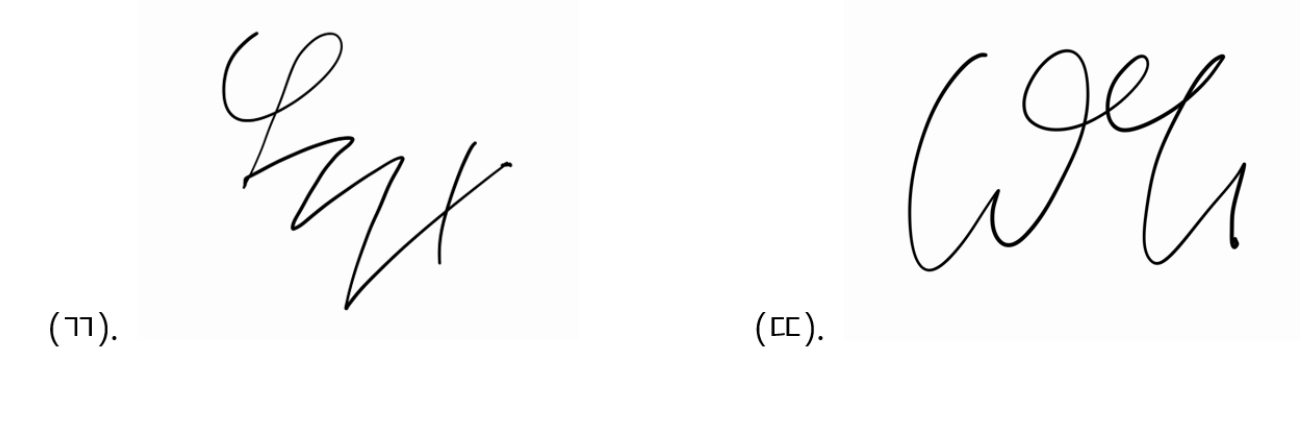
\includegraphics[width=0.75\textwidth]{assets/p3_cursive.png}
\end{center}

\warnnote 영어는 인도유럽어족에 속한다. 전세계에서 수십억 명이 사용한다. 데저레트 문자는 19세기 중반의 미국식 영어를 기반으로 브리검 영에 의해 개발되었다. 영어 철자 개혁 및 몰몬교에서의 사용이라는 두 가지 목적에 의해 제작되었으며, 현재는 극히 소수의 인원에 의해 사용된다. 이 문제에서 사용하는 영어의 음성 기호 표기는 실제 표기를 간략화한 것이다.
\credit{유승민}

\problem{문제 \#4}
마방진이란 가로세로 칸의 개수가 같은 사각형 표의 각 칸에 숫자들을 가로, 세로, 대각선의 합이 모두 같도록 채워넣은 것을 말한다.

다음은 가로, 세로, 대각선의 합이 모두 15인 3$\times$3 마방진과 합이 모두 70인 4$\times$4 마방진이다. 왼쪽 마방진 2개는 나시오이어 수사로, 오른쪽 마방진 2개는 사보사보어 수사로 채워져 있다. 몇몇 칸은 비거나 아라비아 숫자가 기입되어 있으며, 좌우 마방진의 각 칸에 들어갈 숫자는 동일하다.

\begingroup
\setlength{\tabcolsep}{0pt}
\renewcommand{\arraystretch}{1}
\setlength{\arrayrulewidth}{0.4pt}

% 모든 마방진의 전체 한 변 길이
% 표가 너무 크면 7.8cm 정도로 줄이고, 더 여유 있으면 8.1cm까지 키워도 됨.
\newlength{\MSside}
\setlength{\MSside}{8.0cm}

% 3x3, 4x4 셀 크기: 선 두께까지 고려해서 계산
\newlength{\MScellthree}
\setlength{\MScellthree}{(\MSside - 4\arrayrulewidth) / 3}

\newlength{\MScellfour}
\setlength{\MScellfour}{(\MSside - 5\arrayrulewidth) / 4}

\newcolumntype{M}[1]{>{\centering\arraybackslash}m{#1}}

% 셀 하나. 글자 크기는 줄이지 않고, 현재 본문 크기 그대로 사용함.
% 긴 항목이 있을 때만 줄간격을 약간 조밀하게 함.
\newcommand{\mscell}[2]{%
  \parbox[c][#1][c]{#1}{%
    \centering
    \linespread{0.86}\selectfont
    #2%
  }%
}

\begin{center}
\begin{minipage}[t]{\MSside}
\centering
\textbf{나시오이어 마방진}\par\vspace{0.4em}
\begin{tabular}{|M{\MScellthree}|M{\MScellthree}|M{\MScellthree}|}
\hline
\mscell{\MScellthree}{(1)} &
\mscell{\MScellthree}{paʔnokoʔ keta\\karenaumo ta:} &
\mscell{\MScellthree}{kena:nka} \\
\hline
\mscell{\MScellthree}{be:naumo} &
\mscell{\MScellthree}{5} &
\mscell{\MScellthree}{paʔnokoʔ keta\\kena:nka ta:} \\
\hline
\mscell{\MScellthree}{(2)} &
\mscell{\MScellthree}{naruŋ} &
\mscell{\MScellthree}{(3)} \\
\hline
\end{tabular}
\end{minipage}
\hfill
\begin{minipage}[t]{\MSside}
\centering
\textbf{사보사보어 마방진}\par\vspace{0.4em}
\begin{tabular}{|M{\MScellthree}|M{\MScellthree}|M{\MScellthree}|}
\hline
\mscell{\MScellthree}{aɰava} &
\mscell{\MScellthree}{kuava} &
\mscell{\MScellthree}{endo} \\
\hline
\mscell{\MScellthree}{3} &
\mscell{\MScellthree}{ara} &
\mscell{\MScellthree}{7} \\
\hline
\mscell{\MScellthree}{kui} &
\mscell{\MScellthree}{(4)} &
\mscell{\MScellthree}{poɰoa} \\
\hline
\end{tabular}
\end{minipage}
\end{center}

\vspace{1.2em}

\begin{center}
\begin{minipage}[t]{\MSside}
\centering
\begin{tabular}{|M{\MScellfour}|M{\MScellfour}|M{\MScellfour}|M{\MScellfour}|}
\hline
\mscell{\MScellfour}{kivora} &
\mscell{\MScellfour}{kena:nka\\kivoraita\\karenaumo\\ta:} &
\mscell{\MScellfour}{(5)} &
\mscell{\MScellfour}{13} \\
\hline
\mscell{\MScellfour}{21} &
\mscell{\MScellfour}{kivoraita\\paʔnokoʔ\\ta:} &
\mscell{\MScellfour}{kivoraita\\paʔnokoʔ\\keta naruŋ\\ta:} &
\mscell{\MScellfour}{(6)} \\
\hline
\mscell{\MScellfour}{(7)} &
\mscell{\MScellfour}{\small kivoraita\\paʔnokoʔ keta\\karenaumo ta:} &
\mscell{\MScellfour}{20} &
\mscell{\MScellfour}{(8)} \\
\hline
\mscell{\MScellfour}{kena:nka\\kivoraita\\kena:nka\\ta:} &
\mscell{\MScellfour}{(9)} &
\mscell{\MScellfour}{kivoraita\\naruŋ ta:} &
\mscell{\MScellfour}{(10)} \\
\hline
\end{tabular}
\end{minipage}
\hfill
\begin{minipage}[t]{\MSside}
\centering
\begin{tabular}{|M{\MScellfour}|M{\MScellfour}|M{\MScellfour}|M{\MScellfour}|}
\hline
\mscell{\MScellfour}{atale} &
\mscell{\MScellfour}{(11)} &
\mscell{\MScellfour}{nebolo\\iɰiva} &
\mscell{\MScellfour}{(12)} \\
\hline
\mscell{\MScellfour}{nebolo pa} &
\mscell{\MScellfour}{aranipiti} &
\mscell{\MScellfour}{(13)} &
\mscell{\MScellfour}{kuinipiti} \\
\hline
\mscell{\MScellfour}{\small poɰoronipiti} &
\mscell{\MScellfour}{(14)} &
\mscell{\MScellfour}{(15)} &
\mscell{\MScellfour}{14} \\
\hline
\mscell{\MScellfour}{nebolo\\endo} &
\mscell{\MScellfour}{12} &
\mscell{\MScellfour}{Panipiti} &
\mscell{\MScellfour}{nebolo\\ara} \\
\hline
\end{tabular}
\end{minipage}
\end{center}
\endgroup

\vspace{0.9em}

빈칸 (1)$\sim$(15)을 해당 마방진에 사용된 언어로 채워라.

\vspace{0.9em}

\warnnote 나시오이어는 남부건빌어족에 속하며, 파푸아뉴기니 남쪽 부건빌 제도에서 약 20,000명이 사용한다. 사보사보어는 중앙솔로몬어족에 속하며, 솔로몬 제도의 사보 섬에서 약 2,400명이 사용한다. ʔ, ŋ, ɰ는 자음이다. 나시오이어의 기호 :는 앞의 모음이 길게 소리남을 뜻한다. 이 문제에 등장하는 수는 25를 초과하지 않는다.
\credit{정원준}

\problem{문제 \#5}
다음은 팅링어 문장과 간단한 행간 주석, 그리고 그 한국어 번역이다.

\noindent\rule{\textwidth}{0.4pt}

\begin{center}
\exampleblock{ke nrââ odho kafe}{2 - 2 - 32 - 21}{2단수 - 원하다 - 마시다 - 커피}{`넌 커피가 마시고 싶어.'}
\hfill
\exampleblock{ha nrî guha nrâ ri varaha}{3 - 2 - 32 - 2 - 2 - 321}{말하다 - ..로 - 언어 - 소유 - 1복수 - 이렇게}{`이렇게 우리 언어로 말해.'}

\vspace{0.9em}
\exampleblock{nrâ yùrrù farrawa nrî sarra nrâ toni}{2 - 32 - 322 - 2 - 32 - 2 - 21}{3단수 - 자르다 - 빵 - ..로 - 칼 - 주어 - 토니}{`토니(Tony)가 칼로 빵을 자르네.'}
\hfill
\exampleblock{nrâ êê nrâ nyoorre}{2 - 4 - 2 - 21}{3단수 - 불타다 - 주어 - 장소}{`그곳이 불타버렸어?'}

\vspace{0.9em}
\exampleblock{wiri fwirri rò veharru}{22 - 32 - 2 - 321}{2복수 - 듣다 - 1단수 - 잘}{`너희들, 내 말 잘 들어.'}
\hfill
\exampleblock{nrâ fi pwere trùyù e}{2 - 3 - 22 - 21 - 4}{3단수 - 가다 - ..에 - 바다 - 의문}{`그는 바다에 갔어, 그렇지?'}

\vspace{0.9em}
\exampleblock{ke troa nrîfa}{2 - 42 - 21}{2단수 - 떠나다 - 오늘}{`너 오늘 떠나?'}
\hfill
\exampleblock{ke nrââ hara ne}{2 - 2 - 32 - 1}{2단수 - 원하다 - 먹다 - 무엇}{`무엇을 먹고 싶어?'}

\vspace{0.9em}
\exampleblock{tòwò kafe tê toni}{32 - 32 - 2 - 31}{따다 - 커피 - ..와 - 토니}{`토니(Tony)와 함께 커피 콩을 따렴.'}
\hfill
\exampleblock{nrâ nrâ treu mê mwagi e}{2 - 2 - 22 - 3 - 21 - 4}{3단수 - 진행 - 다시 - 오다 - 다시 - 의문}{`그는 다시 오고 있어, 그렇지?'}
\end{center}

\noindent\rule{\textwidth}{0.4pt}

각 문장마다 주어진 숫자는 팅링어의 억양을 표현한 것으로, 1이 가장 소리가 낮고 4가 가장 소리가 높다. 팅링어는 단모음과 장모음의 구분이 있으며, 장모음은 하나의 모음으로 취급된다. 같은 모음 글자를 연이어 쓴 것이 장모음을 표현한 것이다.
\vspace{0.9em}

다음 문장들은 억양이 주어져 있지 않다. 빈칸 \blankko{ㄱ}$\sim$\blankko{ㅇ}을 채워넣어라.

\noindent\rule{\textwidth}{0.4pt}

\begin{center}
\exampleblock{ke gûwû hara warra}{\blankko{ㄱ}}{2단수 - 지속 - 먹다 - 아직}{`너 아직도 먹고 있어?'}
\hfill
\exampleblock{nrâ ta jaa}{\blankko{ㄴ}}{3단수 - 때리다 - 누구}{`그가 누구를 때린 거야?'}

\vspace{0.9em}
\exampleblock{rri hô nrâ mêwe e}{\blankko{ㄷ}}{3복수 - 노래하다 - 주어 - 새 - 의문}{`새들이 노래하네, 그렇지?'}
\hfill
\exampleblock{u fâ nrî arrebo nrîfa}{\blankko{ㄹ}}{1단수 - 벽을.짓다 - 도구 - 돌 - 오늘}{`오늘 내가 돌로 벽을 지었어.'}

\vspace{0.9em}
\exampleblock{nrâ hôdrô mwâ nrî nre nrâ nrû e}{\blankko{ㅁ}}{3단수 - 불태우다 - 오두막 - ..로 - 불 - 소유 - 2단수 - 의문}{`그가 불씨로 너의 오두막을 불태웠어, 그렇지?'}
\hfill
\exampleblock{voo wiri fi nrî wake}{\blankko{ㅂ}}{남자들 - 2복수 - 가다 - ..하러 - 일하다}{`거기 남정네들, 일하러 가라고.'}

\vspace{0.9em}
\exampleblock{ke hara nraasi veti}{\blankko{ㅅ}}{2단수 - 먹다 - 쌀 - 많이}{`쌀을 많이 먹어라.'}
\hfill
\exampleblock{u treu jorri mwagi rroto}{\blankko{ㅇ}}{1단수 - 다시 - 보다 - 다시 - 자동차}{`내가 자동차를 다시 보네.'}
\end{center}

\noindent\rule{\textwidth}{0.4pt}

\warnnote 팅링어는 오스트로네시아어족 말레이-폴리네시아어파에 속하며, 누벨칼레도니에서 약 600명이 사용한다.
\credit{김강래}

\end{spacing}
\end{document}
